\documentclass[oneside]{report}

\usepackage{
	amsmath, amssymb, tcolorbox, fancyhdr, enumitem, float,
	graphicx, amsthm, listings, xcolor, hyperref, nicematrix,
	titlesec, tcolorbox, tikz, lipsum
}
\tcbuselibrary{breakable}
\tcbuselibrary{skins}

% Page Layout
\usepackage[a4paper, top=1.2in, bottom=1.2in, inner=1.0in, outer=1.0in]{geometry}

% Font
\usepackage[sc]{mathpazo}

% Title
\title{Assignment 2: CS215}
\author{
    Satyam Sinoliya, 23B0958 \\
    Vaibhav Singh, 23B1068 \\
    Shaik Awez Mehtab, 23B1080
}
\date{}

% Header and Footer
\fancypagestyle{mystyle}{
    \fancyhf{} 
    \fancyhead[L]{\textbf{Assignment 2}} % Text above the line
    \fancyhead[C]{\thepage}
    \fancyhead[R]{\textbf{CS215}}
    \renewcommand{\headrulewidth}{0.4pt}

    \fancyfoot[L]{\textbf{Awez}}
    \fancyfoot[C]{\textbf{Vaibhav}}
    \fancyfoot[R]{\textbf{Satyam}}
    \renewcommand{\footrulewidth}{0.4pt}
}
\pagestyle{mystyle}

% Solution box
\newtcolorbox[
    auto counter,
]{solution}{skin=enhanced,drop shadow,breakable,title=Solution~\thetcbcounter}

% Extra commands
\newcommand{\Ber}{\text{Ber}}
\newcommand{\Bin}{\text{Bin}}
\newcommand{\NegBin}{\text{NegBin}}
\newcommand{\Geo}{\text{Geo}}
\newcommand{\E}{\mathbb{E}}

\begin{document}

\maketitle

\section{Parking lot problem}
\subsection{Part a)}
The MAPE and MASE of the model for the testing dataset is as follows:
\begin{itemize}[noitemsep]
	\item MAPE:  5.349685330136059
	\item MASE:  0.6598538430731961
\end{itemize}


\subsection{Part b)}
The MAPE and MASE of the model for the testing dataset is as follows:
\begin{itemize}[noitemsep]
	\item MAPE:  9.81429557710239
	\item MASE:  0.26311286911247267
\end{itemize}

\subsection{Part c)}
We have used the following smoothing techniques and the following results are achieved:
\begin{itemize}
	\item MAPE:  3.2338475891165857
	\item MASE:  0.17231581778569224
\end{itemize}

\begin{solution}
	% Fill you solution here
	\tcbsubtitle{Task A}
	\textbf{To prove: }\\
	\emph{Let $X$ be a continuous real-valued random variable with CDF  : $\mathbb{R} \rightarrow [0, 1]$. Assume that
	$F_X$ is invertible. Then the random variable $Y := F_X (X) \in [0, 1]$ is uniformly distributed in $[0, 1]$}\\
	\textbf{Proof:}\\
	$F_X$ by definition can also be written as
	\[F_X(x) = P(X\leq x)\]
	Define a new random variable $Y$,
	\[Y =F_X(X) \]
	Y is the result of applying CDF $F_X$ to the random variable $X$.
	To prove the theorem, assume $y\in [0,1]$. So, the probablity that $Y \leq y$ is:
	\[P(Y\leq y) = P(F_X(X)\leq y)\]
	It is assumed that $F_X(x)$ is invertible, so,
	\[P(Y\leq y) = P(X\leq F_X^{-1}(y))\]
	which is basically, probablity that $X$ is less that or equal to $F_X^{-1}(y)$. This can be written in the CDF form, which is $F_X(F_X^{-1}(y))$. So,
	\[P(Y\leq y) = P(X\leq F_X^{-1}(y)) = F_X(F_X^{-1}(y)) = y\]
	So,
	\[P(Y\leq y) = y\]
	where $y\in [0,1]$, which is the CDF of uniform distributon in $[0,1]$.
	So, Y is a uniform distributon in $[0,1]$ regardless of $X$.

	
\end{solution}

% Start writing your answer from here, if you want to use new packages/change something do it in main.tex
\begin{que}
		\textbf{3.1} Let $Q_{1}$, $Q_{2}$ be non-negative random variables. Let $P(Q_1 < q_1) \geq 1-p_1$ and $P(Q_2 < q_2) \geq 1-p_2$
		where $q_1, q_2$ are non-negative. Then show that $P(Q_1Q_2 < q_1q_2) \geq 1 - (p_1 + p_2)$\\
		\textbf{3.2} Given n distinct values ${\{x_i\}}^n_{i=1}$ with mean $\mu$ and standard deviation $\sigma$, prove that for all $i$,
		we have $|x_i - \mu| \leq \sigma \sqrt[]{n-1}$. How does this inequality compare with Chebyshev's inequality as n
		increases? (give an informal answer)
	

	\hspace*{\fill} [5 marks]
\end{que}

\begin{tcolorbox}[breakable]
	\begin{sol}
		\textbf{3.1}Define two events, $E_1$ and $E_2$:
		\begin{enumerate}
			\item $E_1=\{Q_1<q_1\}$
			\item $E_2=\{Q_2<q_2\}$
		\end{enumerate}
		So,
		\[P(E_1)\geq 1-p_1\]
		\[P(E_2)\geq 1-p_2\]
		We need to prove that,
		\[ P(Q_1Q_2 < q_1q_2) \geq 1 - (p_1 + p_2)\]
		Let's define another event $E_3$, where $E_3=\{Q_1Q_2 < q_1q_2\}$\\
		If we consider the complement of $E_3$, which is
		\[\{Q_1Q_2 < q_1q_2\}^\complement=\{Q_1Q_2 \geq q_1q_2\}\]
		\[E_3^\complement=\{Q_1Q_2 \geq q_1q_2\}\]
		\clearpage
		If $Q_1Q_2 \geq q_1q_2$, and $Q_1,Q_2$ are non-negative integers, it is very clear that, atleast one of the following has to be true:
		\[Q_1\geq q_1 \text{ or }Q_2\geq q_2 \]
		This means \[E_3^\complement \subseteq \{Q_1\geq q_1\}\cup\{Q_2\geq q_2\} \]
		This implies,
		\[P(E_3^\complement)\leq P(\{Q_1\geq q_1\}\cup\{Q_2\geq q_2\} )\]
		\[P(E_3^\complement)\leq P(\{Q_1\geq q_1\})+P(\{Q_2\geq q_2\} )\]
		It is clear that:
		\[\{Q_1\geq q_1\} = E_1^\complement \text{ and } \{Q_2\geq q_2\} = E_2^\complement\]
		So,
		\[1-P(E_3)\leq P(E_1^\complement) + P(E_2^\complement)\]
		\[1-P(E_3)\leq 1-P(E_1) + 1-P(E_2)\]
		\[1-P(E_3)\leq 1-(1-p_1) + 1-(1-p_2)\]
		\[1-P(E_3)\leq p_1 +p_2\]
		This implies,
		\[P(E_3)\geq 1-(p_1+p_2)\]
		\textbf{3.2} We know that,
		\[\frac{\sum^n_{i=0}(x_i-\mu)^2}{n-1}=\sigma^2\]
		This implies,
		\[\sum^n_{i=0}(x_i-\mu)^2 = \sigma^2(n-1)\]
		For any $i$,
		\[(x_i-\mu)^2\geq0\]
		So, for each $i$,
		\[(x_i-\mu)^2\leq\sigma^2\times(n-1)\]
		Again, as both $(x_i-\mu)^2$ and $\sigma^2\times(n-1)$ are greater than or equal to zero, we can take square root on both sides.
		\[\sqrt[2]{(x_i-\mu)^2}\leq\sqrt[2]{\sigma^2(n-1)}\]
		\[|x_i-\mu|\leq\sigma\sqrt[]{n-1}\]


	\end{sol}
\end{tcolorbox}

\section{Non-parametric regression}

\subsection{Report Bandwidth Corresponding to Minimum Estimated Risk}

After running the Nadaraya-Watson kernel regression using the Epanechnikov and Gaussian kernel and performing cross-validation for bandwidth selection, the optimal bandwidth corresponding to the minimum estimated risk is:


\begin{itemize}
	\item Optimal Bandwidth of \textbf{Gaussian} kernel: 0.180
	\item Optimal Bandwidth of \textbf{Epanechnikov} kernel: 0.164
\end{itemize}


\subsection{Similarities and Differences Due to Choice of Different Kernel Functions}

\subsubsection{Similarities}
\begin{itemize}
	\item \textbf{General Functionality:} Both kernels assign weights to
	      data points based on their distance from the query point, resulting
	      in similar predictions in regions with high data density.
	\item \textbf{Smoothing:} As the bandwidth increases, all kernel
	      functions produce smoother estimates. At very large bandwidths, all
	      kernels oversmooth the data, giving too much influence to distant
	      points.
	\item \textbf{Cross-validation Behavior:} Both kernels display a
	      similar behavior during cross-validation, and the corresponding
	      risk curves follow the same trend with bandwidth changes.
\end{itemize}

\subsubsection{Differences}
\begin{itemize}
	\item \textbf{Shape of the Weights:}
	      \begin{itemize}
		      \item \textbf{Epanechnikov Kernel:} This kernel assigns
		            zero weight to points farther than the bandwidth due
		            to its quadratic form, creating a more localized
		            effect.
		      \item \textbf{Gaussian Kernel:} This kernel assigns
		            non-zero weight to every point, regardless of
		            distance, due to its exponential decay. It results in
		            smoother estimates, but it is more sensitive to
		            distant points.
	      \end{itemize}

	\item \textbf{Sensitivity to Outliers:}
	      \begin{itemize}
		      \item \textbf{Epanechnikov Kernel:} This kernel is more
		            resilient to outliers because they assign zero or
		            reduced weight to distant points, decreasing the
		            influence of outliers on the prediction.
		      \item \textbf{Gaussian Kernel:} The Gaussian kernel is
		            more prone to incorporating outliers, as it assigns
		            non-zero weights even to far-away points, making it
		            less resilient in the presence of outliers.
	      \end{itemize}
	\item \textbf{Plots}
	      \begin{itemize}
		      \item \textbf{Epanechnikov Kernel:} This kernel produces
		            more precise and localized estimates, with a good
		            balance between bias and variance when using the
		            optimal bandwidth.
		      \item \textbf{Gaussian Kernel:} The Gaussian kernel leads
		            to smoother curves but gives undue influence to
		            distant points, which can result in overfitting or
		            oversmoothing depending on the bandwidth.
	      \end{itemize}
\end{itemize}
Graphs in the next page.
\begin{figure}[H]
	\centering
	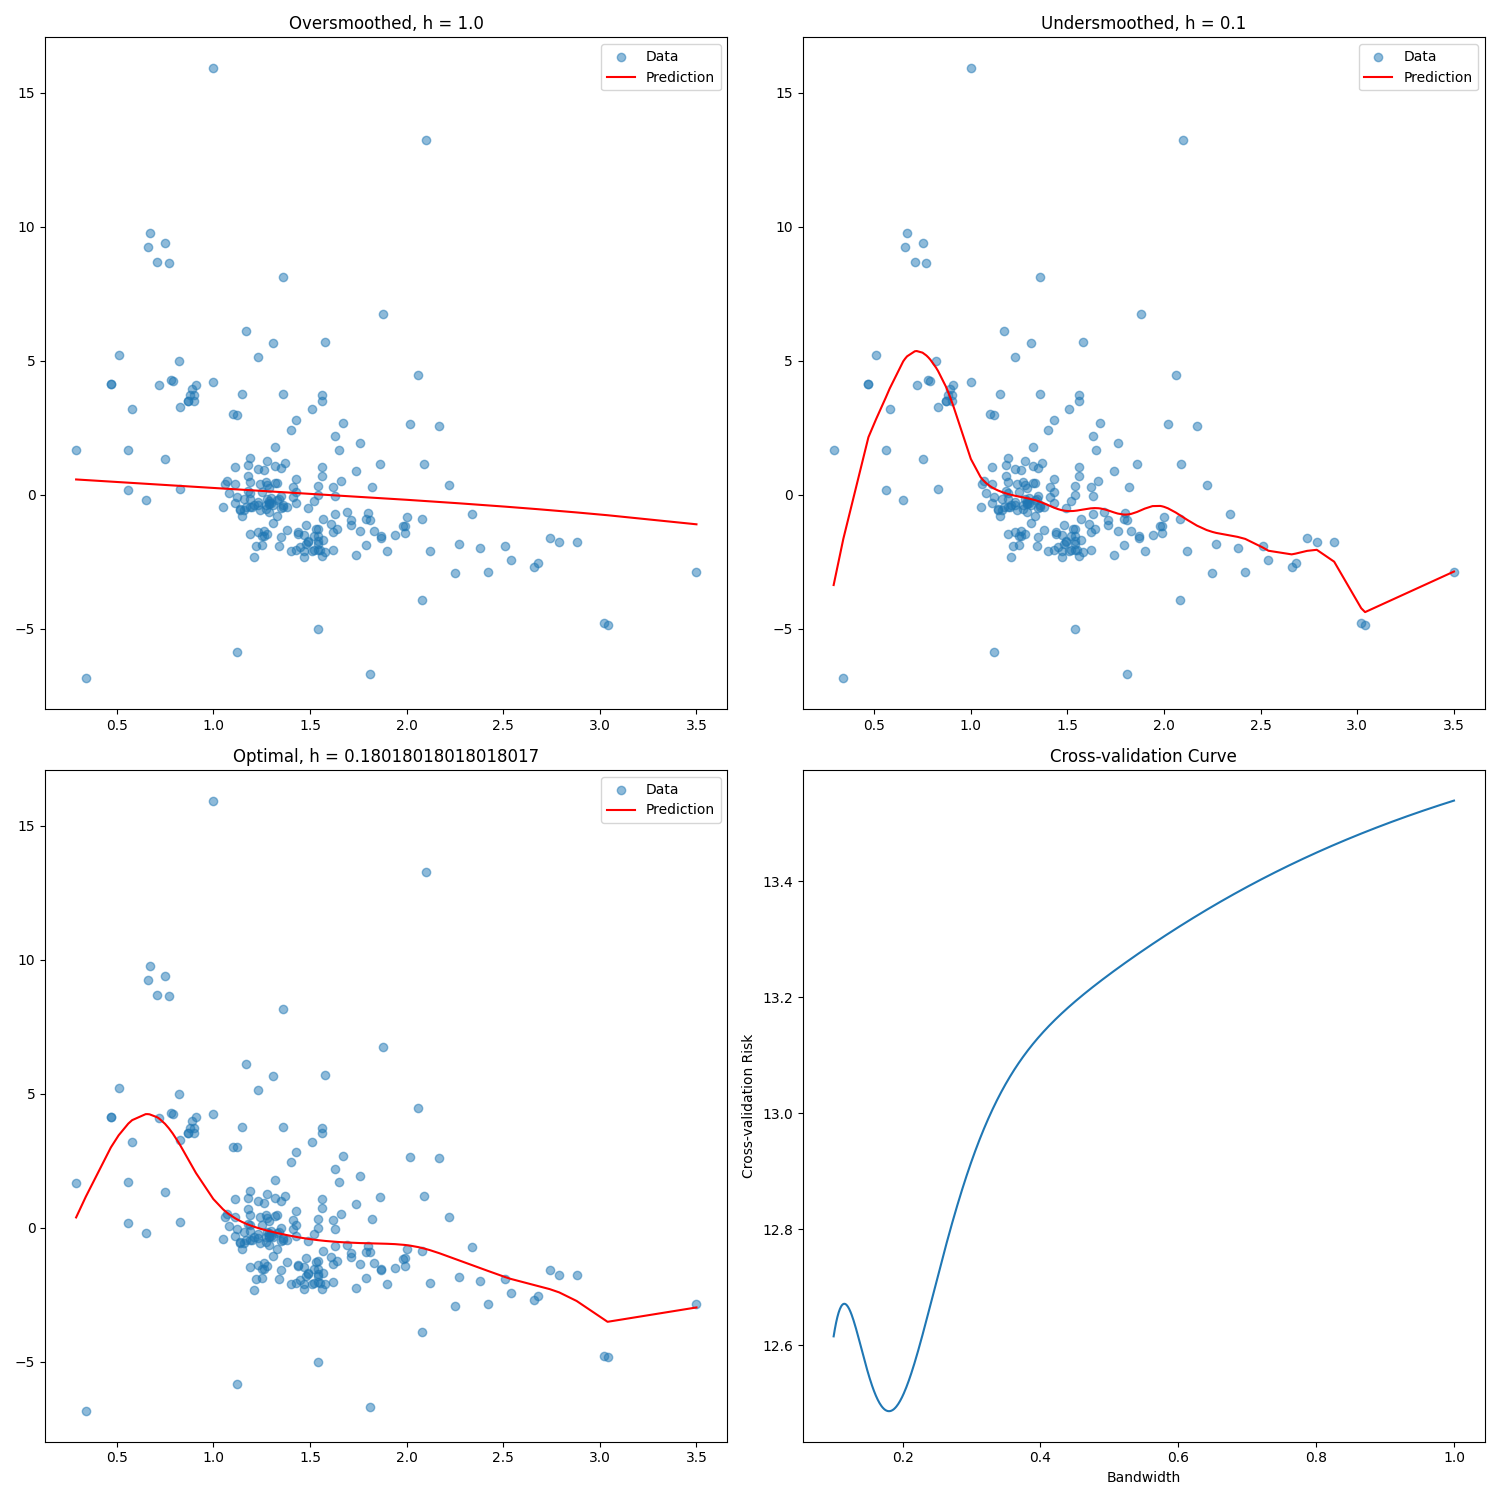
\includegraphics[width=0.5\textwidth]{../images/4/gaussian_kernel_regression.png}
	\caption{Oversmoothed, undersmoothed, optimal and cross validation curve of gaussian kernel}
\end{figure}

\begin{figure}[H]
	\centering
	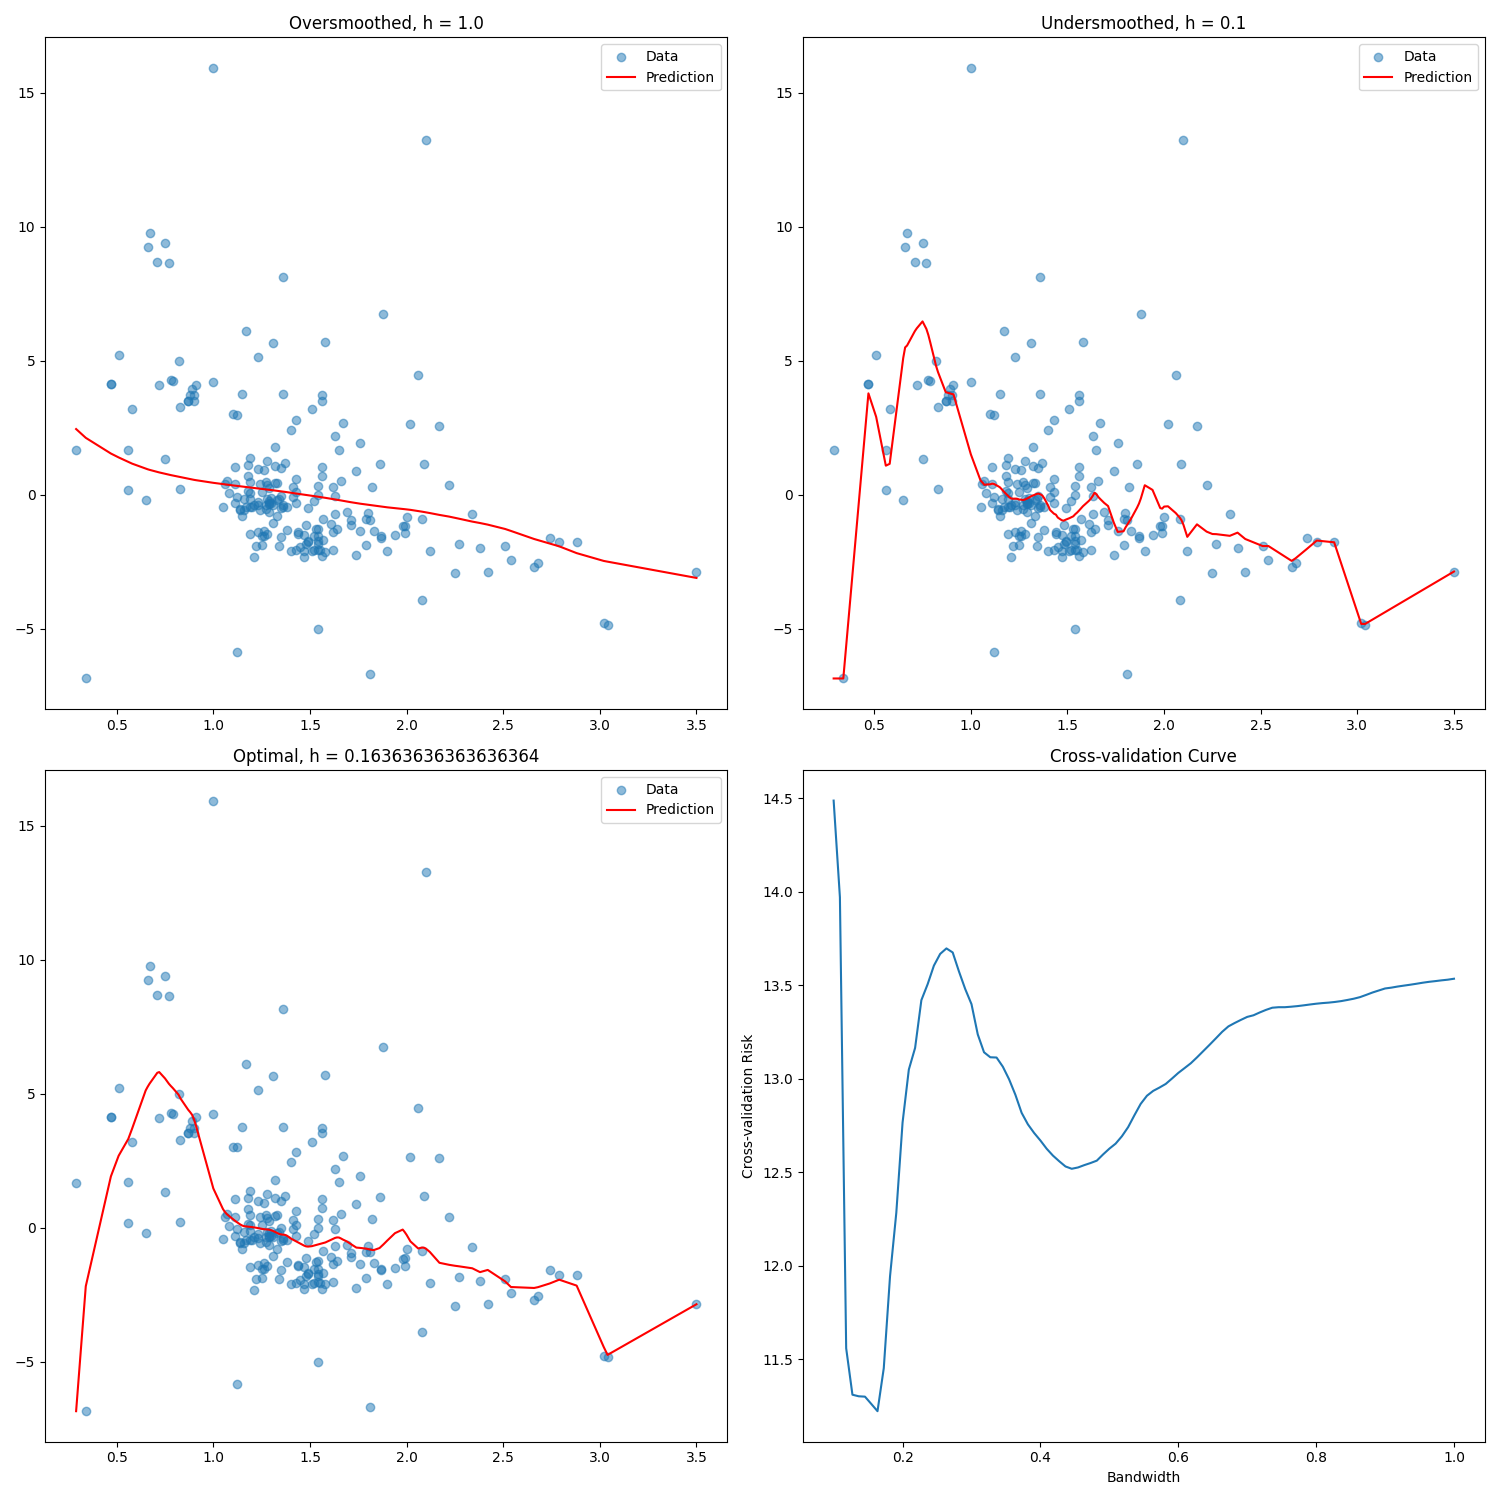
\includegraphics[width=0.5\textwidth]{../images/4/epanechnikov_kernel_regression.png}
	\caption{Oversmoothed, undersmoothed, optimal and cross validation curve of epanechnikov kernel}
\end{figure}

\begin{solution}

	\tcbsubtitle{Task A}

	Given, PDF of GMM variable $X$ is $f_X = \sum_{i=1}^K p_iP[X_i=x]$. Let
	it's CDF be $F_X$. Then $F_X(x)$ is given by

	\begin{align}
		F_X(x) & = P[X\leq x]                                    \\
		       & = \int_{-\infty}^{x} f_X(t)dt                   \\
		       & = \int_{-\infty}^{x} \sum_{i=1}^K p_iP[X_i=t]dt \\
		       & = \sum_{i=1}^K p_i\int_{-\infty}^{x} P[X_i=t]dt \\
		       & = \sum_{i=1}^K p_iP[X_i\leq x]                  \\
		       & = \sum_{i=1}^K p_iF_{X_i}(x)
	\end{align}
	Where $F_{X_i}(x) = P[X_i\leq x]$ is CDF of $X_i$.

	Now, let CDF of output of the given algorithm be
	$F_\A(x) = P[\A\leq x]$. Since the events that we choose $\A$ to be
	from the distribution $i$ (say $E_i$) are disjoint for $i=1,\dots,k$.
	\begin{align}
		F_\A(x) & = P[\A\leq x]                                \\
		        & = \sum_{i=1}^K P[E_i]\cdot P[\A\leq x | E_i] \\
		        & = \sum_{i=1}^K p_iF_{X_i}(x)                 \\
		        & = F_X(x)
	\end{align}

	We know that PDF of a random variable $X$ with CDF $F_X(x)$ is
	$\frac{\partial F_X}{\partial x}$. Thus,
	\begin{align}
		f_\A(x) & = \frac{\partial F_\A}{\partial x} \\
		        & = \frac{\partial F_X}{\partial x}  \\
		        & = f_X
	\end{align}

	Since $x$ was arbitrary, for every $u\in\mathbb{R}$, $f_\A(u) =
		f_X(u)$. i.e the algorithm indeed samples from the GMM variable's
	distribution.


	\tcbsubtitle{Task B}

	Since
	\begin{align}
		\E[X] & = \int_{-\infty}^{\infty} t\cdot P[X=t]dt                    \\
		      & = \int_{-\infty}^{\infty} t\cdot \sum_{i=1}^K p_iP[X_i=t] dt \\
		      & = \sum_{i=1}^K p_i \int_{-\infty}^{\infty} P[X_i = t] dt     \\
		      & = \sum_{i=1}^K p_i \E[X_i]                                   \\
		      & = \sum_{i=1}^K p_i\mu_i
	\end{align}

	Let $\mu = \E[X]$.
	\begin{align}
		\Var[X] & = \int_{-\infty}^{\infty} (t-\mu)^2 P[X=t] dt                    \\
		        & = \int_{-\infty}^{\infty} (t-\mu)^2 \sum_{i=1}^K p_iP[X_i=t] dt  \\
		        & = \sum_{i=1}^K p_i \int_{-\infty}^{\infty} (t-\mu)^2 P[X_i=t] dt \\
		        & = \sum_{i=1}^K p_i \Var[X_i]                                     \\
		        & = \sum_{i=1}^K p_i\sigma_i^2
	\end{align}

	Let $\sigma^2 = \Var[X]$.
	\begin{align}
		\MGF_X(t) & = \int_{-\infty}^{\infty} e^{tX}P[X=x]dx                     \\
		          & = \int_{-\infty}^{\infty} e^{tX} \sum_{i=1}^K p_iP[X_i=x] dx \\
		          & = \sum_{i=1}^K p_i \int_{-\infty}^{\infty} e^{tX}P[X_i=x] dx \\
		          & = \sum_{i=1}^K p_i\MGF_{X_i}(t)                              \\
		          & = \sum_{i=1}^K p_i e^{t\mu_i + \frac{1}{2}t^2\sigma_i^2}
	\end{align}

	\tcbsubtitle{Task C}
	Given $Z=\sum_{i=1}^Kp_iX_i$, where $X_i\sim\N(\mu_i,\sigma_i^2)$

	\begin{align}
		\E[Z] & = \E\left[\sum_{i=1}^Kp_iX_i\right] \\
		      & = \sum_{i=1}^Kp_i\E[X_i]            \\
		      & = \sum_{i=1}^Kp_i\mu_i
	\end{align}

	% \begin{align}
	% 	\Var[Z] & = \Var[\sum_{i=1}^Kp_iX_i]    \\
	% 	        & = \sum_{i=1}^Kp_i^2\Var[X_i]  \\
	% 	        & = \sum_{i=1}^Kp_i^2\sigma_i^2
	% \end{align}
\end{solution}

\end{document}
